\subsection{Kaartweergave werkzaamheden en projecten}\label{kaart}
\pvelist{ \pve{4.27} }
Op \drupalpath{/projecten} is een kaart te vinden met de gepubliceerde projecten en werkzaamheden. Deze projecten kunnen in de backend ook worden gevonden als project nodes\seeone{projectnode}.

De kaart heeft voor de bezoeker de volgende functionaliteit:
\begin{itemize}
\item Alle (door ProRail beheerde) sporen zijn zichtbaar
\item In- en uitzoomen d.m.v. zoomslider of door dubbelklik (beperkte zoomniveau's)
\item Positie veranderen door:
\begin{itemize}
\item knoppen met pijltjes,
\item pijltjestoetsen op het toetsenbord,
\item verslepen met de muis of;
\item verslepen d.m.v. touch navigatie (alleen iPad)
\end{itemize}
\item Popup bij het aanklikken van stations en sporen waar werkzaamheden zijn, met link naar de projectpagina
\end{itemize}
Merk op dat er meer detail verschijnt wanneer men verder inzoomt op de kaart. Kleine stations zullen ook niet zichtbaar zijn op hogere zoomniveau's.

Rechts van de kaart kan een legenda worden geplaatst. Deze wordt via Felix neergezet. Hiervoor wordt een redactioneel blok gebruikt met de titel "Projecten legenda". Kies bij het plaatsen voor "volledige inhoud" als weergave modus.

\subsubsection{Projecten op de kaart beheren}

Bij het toevoegen en bewerken van project nodes zijn een aantal velden beschikbaar die van invloed zijn op de projectenkaart:
\begin{itemize}
\item Keuze soort project
\item Keuze wat in selectie opgenomen moet worden ("Markeren")
\item Kaart met bewerkopties (invoerkaart)
\end{itemize}
\begin{center}
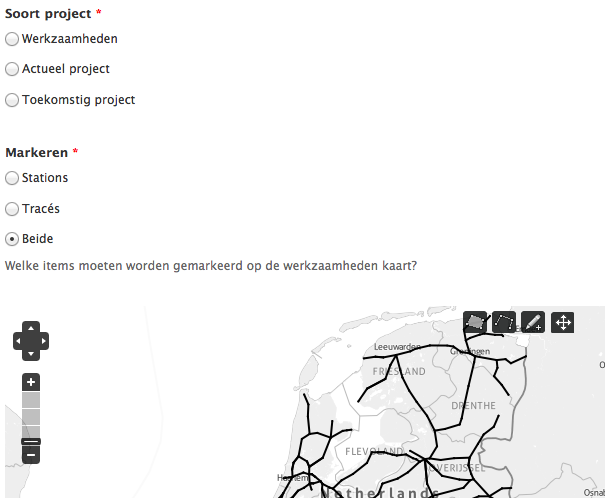
\includegraphics[scale=.5]{img/kaart1.png}
\end{center}
De eerste keuze bepaald de kleur op de kaart. De tweede optie bepaald samen met de selectie op de invoerkaart wat te zien zal zijn op de projectenkaart. Op de invoerkaart kunnen gebieden worden geselecteerd waarbinnen stations en/of trac\'{e}s vallen. De keuze "stations" zal alleen markers bij de stations plaatsen, de keuze "trac\'{e}s" zal alleen de sporen inkleuren en "beide" geeft beide als resultaat.

\paragraph{Nieuw gebied selecteren}
Om een selectie te maken moet eerst worden ingezoomd naar het gebied waar de selectie moet worden gemaakt. Hoever precies wordt ingezoomd is niet relevant, maar zo ver mogelijk inzoomen maakt de selectie makkelijker. Tevens verschijnen dan de locaties van de stations. Inzoomen werkt op de invoerkaart hetzelfde als op de projectenkaart. Rechtsboven staan 4 knoppen die gebruikt worden om de selectie te maken. Klik op de linkerknop. Deze knop is voor het selecteren van een gebied. Om iets te selecteren wat al op de kaart staat moet altijd een gebied worden gebruikt, dus ook als het om een enkel station gaat.
%\begin{center}
%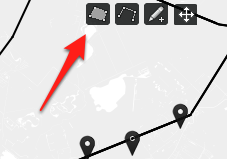
\includegraphics[scale=.7]{img/kaart2.png}
%\end{center}
De actieve knop is grijs wanneer deze actief is. De werkelijke selectie kan nu worden gemaakt. Klik hiervoor op de positie van \'{e}\'{e}n van de hoeken. Klik daarna achtereenvolgend op de volgende hoeken. Voor alle hoeken wordt een enkele klik gebruikt behalve voor de laatste hoek. Dubbelklikken zorgt ervoor dat de vorm gesloten wordt en geeft dus aan dat we klaar zijn met de selectie van dit gebied. De vorm blijft nu staan.
\begin{center}
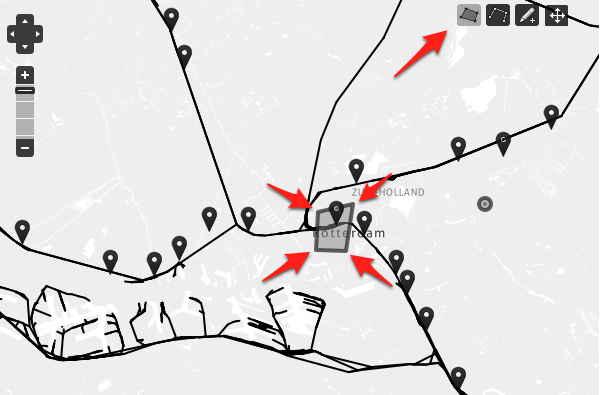
\includegraphics[scale=.7]{img/kaart3.png}
\end{center}
Als de selectie zo goed is dan kan de node worden opgeslagen. Let hierbij op de workflow, alleen gepubliceerde nodes komen op de projectenkaart. Na het opslaan van de node worden de kaartgegevens direct bijgewerkt. De voortgang wordt getoond. Dit zal doorgaans niet meer dan 10 seconden duren. Het project is daarna meestal direct te zien, maar de weergave kan door omstandigheden (browser caching) maximaal 2 minuten vertraagd zijn.
\begin{center}
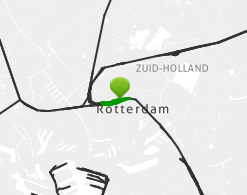
\includegraphics[scale=.7]{img/kaart4.png}
\end{center}
Afhankelijk van de gekozen opties zal er een marker en/of opgelicht spoort te zien zijn in het geselecteerde gebied. Merk op dat het voor kleinere stations nodig kan zijn om verder in te zoomen alvorens deze te zien is. Hierboven is het resultaat weergegeven van de eerder gemaakte selectie, met zowel stations als trac\'{e}s.

Er is geen limiet op het aantal stations en sporen dat een gebied kan bevatten. Het is ook mogelijk om meerdere gebieden te selecteren. Hiervoor kunnen dezelfde stappen nogmaals worden doorlopen.

\paragraph{Selectie aanpassen of verwijderen}

Voor het aanpassen van de selectie moet gebruik worden gemaakt van de vierde knop rechtsboven op de invoerkaart. Klik eerst op deze knop en klik daarna op het gebied dat aangepast of verwijderd moet worden. Na het klikken op het gebied verschijnen cirkels om de hoeken.
\begin{center}
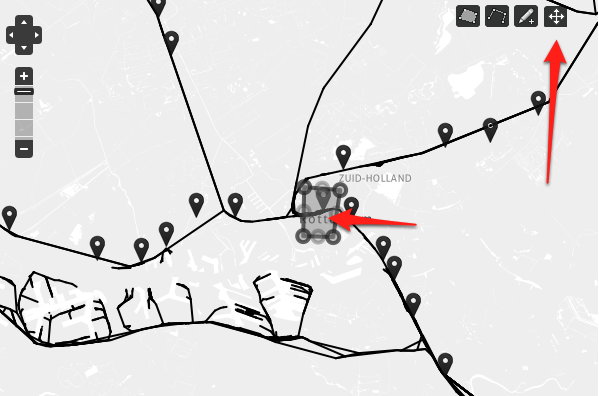
\includegraphics[scale=.7]{img/kaart5.png}
\end{center}
Het is mogelijk om de cirkels om de hoeken te verslepen. Op deze manier kan de vorm worden aangepast. Hiermee kan een eerder gemaakte selectie worden gecorrigeerd, maar het is ook met name handig voor grotere selecties. Op die manier is het namelijk niet noodzakelijk om een selectie meteen de eerste keer goed te tekenen.
\begin{center}
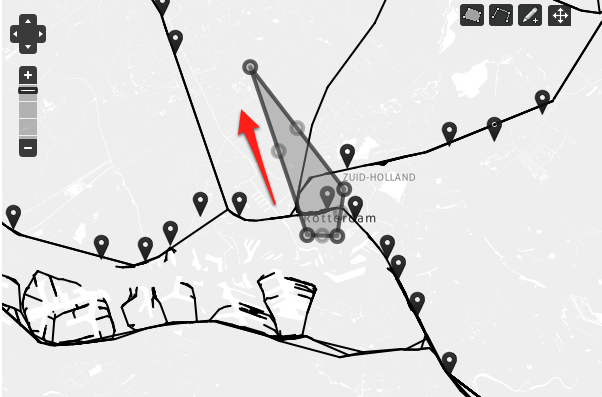
\includegraphics[scale=.7]{img/kaart6.png}
\end{center}
Naast de cirkels rondom de hoeken verschijnen er tevens - in een lichtere tint - cirkels \emph{tussen} de hoeken. Door deze te verslepen 'breekt de lijn' en wordt een extra hoek gecre\"{e}ert.
\begin{center}
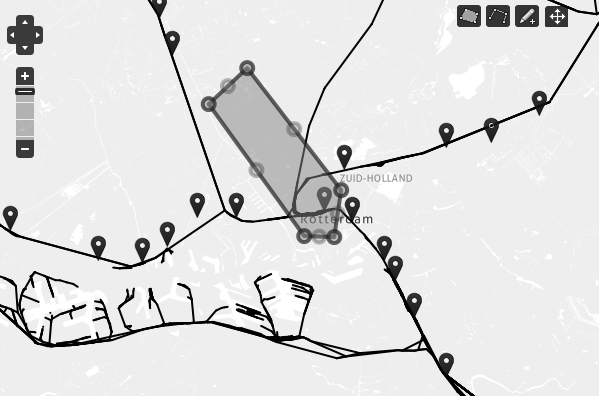
\includegraphics[scale=.7]{img/kaart7.png}
\end{center}
Om een vorm te verwijderen kan de D-toets ("delete") op het toetsenbord worden gebruikt. De geselecteerde vorm zal dan verdwijnen.

\paragraph{Nieuwe trac\'{e}s en markers}

Naast het selecteren van bestaande objecten d.m.v. een gebied is het ook mogelijk om zelf trac\'{e}s en stations / markers op de kaart te plaatsen. Hiervoor zijn de tweede en derde knop rechtsboven op de invoerkaart.

Klik op de tweede knop voor het tekenen van trac\'{e}s. Klik vervolgens op het beginpunt. Daarna kunnen de volgende punten aangeklikt worden. Bij het laatste punt moet dubbel worden geklikt om de selectie te eindigen. De werking is identiek aan het selecteren van een gebied, alleen zal er zich geen gesloten vorm vormen.
\begin{center}
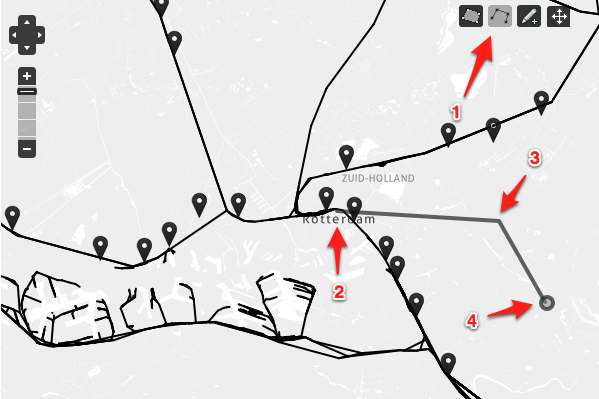
\includegraphics[scale=.7]{img/kaart8.png}
\end{center}
De lijn kan op elk willekeurig punt beginnen. In bovenstaand voorbeeld begint deze op station Rotterdam, maar het is niet noodzakelijk om op enige manier aan te sluiten op de bestaande objecten.

Naast de trac\'{e}s kunnen ook eigen markers worden geplaatst. Klik hiervoor op de derde knop (het potloodje). Klik daarna op de positie waar de marker moet komen. Bij deze optie moet - anders dan de andere vormen - \'{e}\'{e}n keer worden geklikt.
\begin{center}
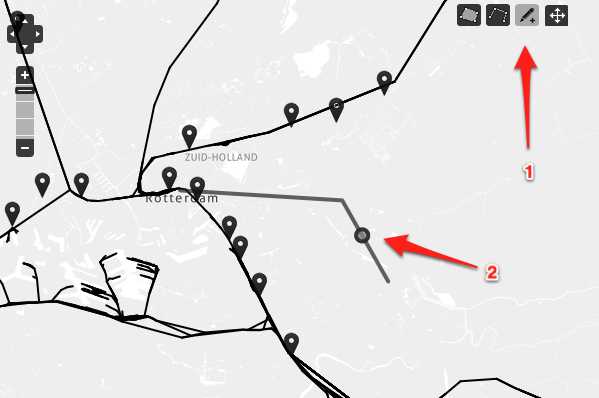
\includegraphics[scale=.7]{img/kaart9.png}
\end{center}
In het voorbeeld hierboven staat de marker ergens halverwege het eerder getekende spoor. Net als bij nieuwe sporen kan deze echter overal op de kaart worden geplaatst. In de afbeelding hieronder is de uitwerking van bovenstaande selectie te zien op de projectenkaart.
\begin{center}
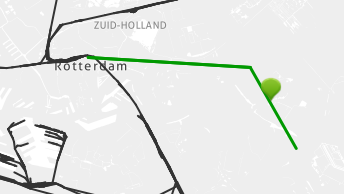
\includegraphics[scale=.7]{img/kaart10.png}
\end{center}

\subsubsection{Tekstueel overzicht kaart}
Het blok \emph{Tekstueel overzicht kaart} dient in PHP modus bewerkt te worden in de WYSIWYG, omdat de link op alle domeinen moet werken.
\drupalpath{/omwonenden/node/2021/edit}

